% ===============================================================
%  جلسه پانزدهم
% ===============================================================
\chapter{توزیع‌های مشترک تکین، گشتاورهای مشترک، کوواریانس و همبستگی}

\section{ادامه بحث متغیرهای مشترکاً گاوسی}

در جلسه قبل دیدیم که دو متغیر $X\sim\mathcal N(\mu,\sigma^2)$ و $Y\sim\mathcal N(\mu',\sigma'^2)$ را مشترکاً گاوسی با ضریب همبستگی $r$ می‌نامیم اگر
\[
f_{X,Y}(x,y)=\frac{1}{2\pi\sigma\sigma'\sqrt{1-r^2}}\exp\left[\frac{-1}{2(1-r^2)}\left(\frac{(x-\mu)^2}{\sigma^2}+\frac{(y-\mu')^2}{\sigma'^2}-2r\frac{(x-\mu)(y-\mu')}{\sigma\sigma'}\right)\right],
\]
و دیدیم که حاشیه‌ها گاوسی‌اند، $r=0$ استقلال را نتیجه می‌دهد، و توزیع شرطی نیز گاوسی است (\textcolor{red!70!black}{اثبات در خانه} ــ که در جلسه قبل با تکمیل مربع انجام دادیم):
\[
X\given Y=y\ \sim\ \mathcal N\Big(\mu+\frac{\sigma}{\sigma'}r(y-\mu'),\ (1-r^2)\sigma^2\Big).
\]

\subsection{حالت حدی $|r|=1$}
در صورتی که ضریب همبستگی خاصیت $|r|=1$ را دارا باشد، واریانس شرطی $(1-r^2)\sigma^2$ صفر می‌شود؛ یعنی در صورت دانستن یکی از متغیرهای تصادفی $X,Y$، مقدار دیگری به صورت \textbf{یقینی} مشخص خواهد شد:
\[
\boxed{\ X=\mu\pm\frac{\sigma}{\sigma'}(y-\mu')\ }
\]
(علامت $+$ برای $r=1$ و علامت $-$ برای $r=-1$.) در صورتی که $X,Y$ هم‌توزیع می‌بودند (یعنی میانگین و واریانس یکسان می‌داشتند)، ضریب همبستگی ۱ به معنی $X=Y$ می‌شد.

\begin{note}
\notetitle در این حالت فرمول چگالی مشترک (که $\sqrt{1-r^2}$ در مخرج دارد) معنا ندارد: کل جرم احتمال روی یک خط در صفحه متمرکز است و چگالی دوبعدی معمولی وجود ندارد. برای توصیف چنین توزیع‌هایی به ابزار بخش بعد ــ «توزیع‌های تکین» ــ نیاز داریم.
\end{note}

\subsection{ترکیب‌های خطی}
متغیرهای تصادفی $X,Y$ در صورتی که مشترکاً نرمال باشند:
\begin{itemize}
\item به ازای هر مقدار $a,b\in\R$، توزیع $aX+bY$ همواره گاوسی است با میانگین $a\mu+b\mu'$ و واریانس $a^2\sigma^2+b^2\sigma'^2+2abr\sigma\sigma'$ (پاسخ پرسش جلسه قبل؛ پایین‌تر با مفهوم کوواریانس دوباره به آن می‌رسیم).
\item به ازای $a,b,c,d\in\R$، دو متغیر $aX+bY$ و $cX+dY$ مشترکاً گاوسی هستند.
\end{itemize}

\section{توزیع‌های مشترک ترکیبی (تکینگی‌های خطی و نقطه‌ای)}

\subsection{توزیع‌های مشترک جرمی}
فرض کنید که متغیرهای تصادفی $X,Y$ هر دو ماهیت گسسته داشته باشند و $\mathrm{supp}(X)=\{x_1,x_2,\ldots\}$ و $\mathrm{supp}(Y)=\{y_1,y_2,\ldots\}$. در این صورت، خواهیم داشت:
\[
\boxed{\ f_{XY}(x,y)=\sum_{x_i,y_j}\Prob(X=x_i,Y=y_j)\,\delta(x-x_i,\ y-y_j)\ }
\]
در اینجا $\delta(x,y)$ نشانگر \textbf{تابع دلتای دیراک دومتغیره} است. تابع $\delta(x,y)$ فقط در نقطه $(0,0)$ غیرصفر بوده و داریم:
\[
\iint_{S\subseteq\R^2}\delta(x,y)\dd x\dd y=\ind_{(0,0)\in S}.
\]
(می‌توان نوشت $\delta(x,y)=\delta(x)\delta(y)$.)

\subsubsection*{توزیع حاشیه‌ای}
دقت کنید که داریم:
\[
\int_{-\infty}^{+\infty}\delta(x,y)\dd y=\delta(x).
\]
در نتیجه توزیع‌های حاشیه‌ای به صورت زیر درخواهند آمد:
\[
\begin{aligned}
f_X(x)&=\int_\R f_{XY}(x,y)\dd y=\sum_{x_i,y_j}\Prob(X=x_i,Y=y_j)\int_\R\delta(x-x_i,y-y_j)\dd y\\
&=\sum_{x_i}\Prob(X=x_i)\,\delta(x-x_i),
\end{aligned}
\]
که در آخرین تساوی، جملات با $x_i$ یکسان را با هم جمع کرده‌ایم ($\sum_j\Prob(X=x_i,Y=y_j)=\Prob(X=x_i)$). این همان \lr{PDF} متغیر گسسته $X$ است که در جلسه هشتم دیدیم.

\subsection{توزیع‌های مشترک خطی}
\begin{definition}[توزیع مشترک خطی]
فرض کنید که متغیر تصادفی $X$ دارای توزیعی دلخواه با چگالی احتمال $f_X(x)$ و متغیر تصادفی $Y$ با اعمال یک تابع یقینی مانند $g$ بر $X$ حاصل شود؛ یعنی داشته باشیم $Y=g(X)$. در این صورت، تابع توزیع مشترک $X,Y$ به صورت زیر در خواهد آمد:
\[
\boxed{\ f_{XY}(x,y)=f_X(x)\,\delta\big(y-g(x)\big)\ }
\]
\end{definition}
\begin{proof}[توجیه]
با قانون زنجیره‌ای $f_{XY}(x,y)=f_X(x)f_{Y|X}(y\given x)$. به شرط $X=x$، متغیر $Y$ به‌طور قطعی برابر $g(x)$ است؛ پس توزیع شرطی آن یک ضربه در $g(x)$ است: $f_{Y|X}(y\given x)=\delta(y-g(x))$.
\end{proof}

\textbf{تصویر شهودی:} یک چگالی مشترک معمولی (مثلاً گاوسی دو متغیره با $|r|$ نزدیک ۱) را در نظر بگیرید. وقتی $|r|\to1$، عرض توزیع (در جهت عمود بر خم) به سمت صفر میل کرده و توزیع حول خم $y=g(x)$ \textbf{تکین} خواهد شد: یک «دیوار» بی‌نهایت نازک و بی‌نهایت بلند روی خم، با حجم کل ۱.

\begin{center}
\begin{tikzpicture}
\begin{axis}[view={0}{90},width=5.6cm,height=5.6cm,xmin=-3,xmax=3,ymin=-3,ymax=3,title={$r=0.5$},xtick=\empty,ytick=\empty,axis equal image]
\addplot3[contour gnuplot={levels={0.03,0.08,0.13},labels=false},thick,samples=40,domain=-3:3,y domain=-3:3] {exp(-(x^2+y^2-1*x*y)/(2*0.75))/(2*pi*sqrt(0.75))};
\end{axis}
\end{tikzpicture}
\begin{tikzpicture}
\begin{axis}[view={0}{90},width=5.6cm,height=5.6cm,xmin=-3,xmax=3,ymin=-3,ymax=3,title={$r=0.95$},xtick=\empty,ytick=\empty,axis equal image]
\addplot3[contour gnuplot={levels={0.05,0.15,0.3},labels=false},thick,samples=60,domain=-3:3,y domain=-3:3] {exp(-(x^2+y^2-1.9*x*y)/(2*0.0975))/(2*pi*sqrt(0.0975))};
\end{axis}
\end{tikzpicture}
\begin{tikzpicture}
\begin{axis}[width=5.6cm,height=5.6cm,xmin=-3,xmax=3,ymin=-3,ymax=3,title={$r=1$ (تکین)},xtick=\empty,ytick=\empty,axis equal image]
\addplot[very thick,red,domain=-3:3] {x};
\end{axis}
\end{tikzpicture}
\end{center}

\subsection{مرتبه تکینگی \lr{(Singularity Level)}}
\begin{itemize}
\item در مورد توزیع‌های مشترک \textbf{خطی}، و بر خلاف توزیع‌های مشترک جرمی، تکینگی تابع \lr{pdf} تنها \textbf{یک مرتبه} (یعنی از مرتبه $\delta(\cdot)$) است:
\[
f_{XY}(x,y)=f_X(x)\,\delta\big(y-g(x)\big).
\]
جرم روی یک \emph{خم} (یک‌بعدی) پخش شده است.
\item یادآوری: تکینگی تابع چگالی احتمال (\lr{pdf}) در مورد توزیع‌های \textbf{جرمی} از \textbf{مرتبه ۲}، یعنی $\delta^2(\cdot)$ است:
\[
f_{XY}(x,y)=\sum_{x_i,y_j}\Prob(X=x_i,Y=y_j)\,\delta(x-x_i)\,\delta(y-y_j).
\]
جرم در \emph{نقاط} (صفربعدی) متمرکز است.
\end{itemize}

\begin{example}[استفاده از چگالی تکین]
$X\sim\mathcal U(0,1)$ و $Y=X^2$. با استفاده از چگالی مشترک تکین، $\E(XY)$ و $f_Y$ را بیابید.
\begin{solution}
$f_{XY}(x,y)=\ind_{[0,1]}(x)\,\delta(y-x^2)$. پس
\[
\E(XY)=\iint xy\,\delta(y-x^2)\ind_{[0,1]}(x)\dd y\dd x=\int_0^1x\cdot x^2\dd x=\frac14
\]
(خاصیت غربالی دلتا، $y$ را با $x^2$ جایگزین می‌کند). برای حاشیه $Y$: $f_Y(y)=\int_0^1\delta(y-x^2)\dd x$. با تغییر متغیر $u=x^2$ ($\dd x=\frac{\dd u}{2\sqrt u}$): $f_Y(y)=\frac{1}{2\sqrt y}$ برای $0<y<1$ ــ همان نتیجه فرمول تبدیل جلسه دوازدهم.
\end{solution}
\end{example}

\section{گشتاورهای مشترک \lr{(Joint Moments)}}

\begin{definition}[گشتاور مشترک]
فرض کنید متغیرهای تصادفی $X,Y$ دارای چگالی احتمال مشترک $f_{XY}$ باشند. در این صورت، گشتاور مرتبه $(m,n)$ از توزیع مشترک $f_{XY}$ را به صورت زیر تعریف می‌کنیم:
\[
m_{m,n}=\E\big(X^mY^n\big)=\iint x^my^nf_{XY}(x,y)\dd x\dd y .
\]
\end{definition}

\subsection{خواص و ویژگی‌ها}
ویژگی‌های ذکر شده در قبل، کماکان به صورت تعمیم‌یافته برقرار هستند:
\[
m_{1,0}=\mu_X\ ,\quad m_{0,1}=\mu_Y,
\qquad
m_{2,0}-m_{1,0}^2=\sigma_X^2\ ,\quad m_{0,2}-m_{0,1}^2=\sigma_Y^2 .
\]
\begin{itemize}
\item \textbf{خاصیت خطی \lr{Expectation}:}
$\E(aX+bY+c)=a\E(X)+b\E(Y)+c$.
\item \textbf{اتحادهای ساده:}
\[
\E\big((X-\mu_X)(Y-\mu_Y)\big)=m_{1,1}-m_{0,1}m_{1,0}=\E(XY)-\E(X)\E(Y).
\]
\end{itemize}
\begin{proof}[اثبات اتحاد آخر]
با بسط ضرب و خاصیت خطی:
$\E(XY-\mu_YX-\mu_XY+\mu_X\mu_Y)=\E(XY)-\mu_Y\mu_X-\mu_X\mu_Y+\mu_X\mu_Y=\E(XY)-\mu_X\mu_Y$.
\end{proof}

\section{کوواریانس و همبستگی آماری}

\begin{definition}[کوواریانس]
به آماره زیر در اصطلاح \textbf{کوواریانس} (\textcolor{red!70!black}{\lr{Covariance}}) دو متغیر تصادفی $X,Y$ اطلاق می‌گردد:
\[
\Cov(X,Y)=C_{X,Y}\triangleq\E\big[(X-\mu_X)(Y-\mu_Y)\big]=\E(XY)-\mu_X\mu_Y .
\]
\end{definition}
کوواریانس، \textbf{میزان تغییرات خطی هم‌زمان} دو متغیر را اندازه‌گیری می‌کند: اگر وقتی $X$ از میانگینش بزرگ‌تر است، $Y$ نیز معمولاً از میانگینش بزرگ‌تر باشد، حاصل‌ضرب $(X-\mu_X)(Y-\mu_Y)$ اغلب مثبت و کوواریانس مثبت است؛ و برعکس.

\begin{definition}[ضریب همبستگی]
به منظور بهنجارسازی و داشتن دید بهتری از رفتار مشابه بین دو متغیر تصادفی، \textbf{ضریب همبستگی} (\textcolor{red!70!black}{\lr{Correlation Coefficient}}) را به صورت زیر تعریف می‌کنیم:
\[
\mathrm{corr}(X,Y)=\rho_{X,Y}\triangleq\frac{\E\big[(X-\mu_X)(Y-\mu_Y)\big]}{\sigma_X\sigma_Y}=\frac{\Cov(X,Y)}{\sigma_X\sigma_Y}.
\]
به این رابطه، \textbf{ضریب همبستگی پیرسون} (\lr{Pearson Correlation Coefficient}) یا \lr{Correlation} هم اطلاق می‌گردد.
\end{definition}

\begin{note}
\notetitle کوواریانس به واحد اندازه‌گیری بستگی دارد (اگر قد را به جای متر با سانتی‌متر بسنجیم، کوواریانس ۱۰۰ برابر می‌شود)، اما ضریب همبستگی بی‌بُعد است و تحت تبدیل‌های خطی $aX+b$ (با $a>0$) تغییر نمی‌کند. خواص مفید کوواریانس: $\Cov(X,X)=\Var X$، $\Cov(X,Y)=\Cov(Y,X)$، $\Cov(aX+b,Y)=a\Cov(X,Y)$ و $\Cov(X+Z,Y)=\Cov(X,Y)+\Cov(Z,Y)$ (دوخطی بودن).
\end{note}

\section{ویژگی‌های ضریب همبستگی}

\begin{theorem}[کران ضریب همبستگی]
ضریب همبستگی $\rho_{XY}$ میان هر دو متغیر تصادفی دلخواه، همواره عددی در بازه $[-1,1]$ خواهد بود؛ یعنی $|\rho_{X,Y}|\le1$.
\end{theorem}
\begin{proof}
اثبات بنا بر نامساوی \lr{Cauchy--Schwarz} است: برای هر دو متغیر $U,V$، $\big(\E(UV)\big)^2\le\E(U^2)\E(V^2)$. (اثبات کوشی--شوارتز: برای هر $t$ حقیقی، $0\le\E\big((U-tV)^2\big)=\E U^2-2t\E(UV)+t^2\E V^2$؛ یک چندجمله‌ای درجه دوم نامنفی بر حسب $t$ باید مُبَیِّن نامثبت داشته باشد: $4(\E UV)^2-4\E U^2\E V^2\le0$.) با قرار دادن $U=X-\mu_X$ و $V=Y-\mu_Y$:
$\Cov(X,Y)^2\le\sigma_X^2\sigma_Y^2$، یعنی $|\rho_{XY}|\le1$.
\end{proof}

\begin{theorem}[همبستگی کامل]
در صورتی که ضریب همبستگی میان دو متغیر برابر با $1$ یا $-1$ شود (\lr{fully-correlated} و یا \lr{fully anti-correlated})، بدین معنی است که یکی از دو متغیر به صورت \textbf{ترکیب خطی} دیگری نوشته می‌شود (با احتمال ۱): $Y=aX+b$ که $a>0$ برای $\rho=1$ و $a<0$ برای $\rho=-1$.
\end{theorem}
\begin{proof}
تساوی در کوشی--شوارتز یعنی مبین صفر است، پس $t_0$ای وجود دارد که $\E\big((U-t_0V)^2\big)=0$؛ یعنی $U=t_0V$ تقریباً حتماً، که همان رابطه خطی بین $X-\mu_X$ و $Y-\mu_Y$ است.
\end{proof}

\begin{theorem}[واریانس جمع و تفریق]
اتحاد زیر در مورد واریانس \textbf{جمع} و \textbf{تفریق} دو متغیر تصادفی همواره برقرار است:
\[
\sigma_{X+Y}^2=\sigma_X^2+\sigma_Y^2+2\rho_{XY}\sigma_X\sigma_Y,\qquad
\sigma_{X-Y}^2=\sigma_X^2+\sigma_Y^2-2\rho_{XY}\sigma_X\sigma_Y .
\]
\end{theorem}
\begin{proof}
$\Var(X\pm Y)=\E\big[\big((X-\mu_X)\pm(Y-\mu_Y)\big)^2\big]=\sigma_X^2+\sigma_Y^2\pm2\Cov(X,Y)$ و $\Cov(X,Y)=\rho_{XY}\sigma_X\sigma_Y$.
\end{proof}

\begin{summarybox}[نکته]
در صورتی که $X,Y$ متغیرهای تصادفی \textcolor{red!70!black}{مشترکاً گاوسی} با میانگین و واریانس دلخواه، و ضریب همبستگی $r$ باشند، همواره داریم $\rho_{XY}=r$. (این را در پاسخ پرسش جلسه قبل نشان دادیم: $\Cov(X,Y)=r\sigma\sigma'$.)
\end{summarybox}

\subsection{ناهمبستگی و استقلال}
\begin{definition}
در صورتی که برای دو متغیر تصادفی $X,Y$ داشته باشیم $\rho_{XY}=0$، این دو متغیر را \textbf{ناهمبسته} (\textcolor{red!70!black}{\lr{Uncorrelated}}) می‌نامیم.
\end{definition}
\begin{itemize}
\item در صورتی که دو متغیر تصادفی \textbf{مستقل} باشند، \textbf{ناهمبسته} نیز خواهند بود (زیرا $\E(XY)=\E X\E Y$).
\item اما در صورتی که دو متغیر تصادفی \textbf{ناهمبسته} باشند، لزوماً \textbf{مستقل} نیستند. استقلال آماری شرط بسیار قوی‌تری نسبت به ناهمبسته بودن است.
\end{itemize}

\begin{example}[ناهمبسته اما وابسته]
$X\sim\mathcal U(-1,1)$ و $Y=X^2$. نشان دهید $X,Y$ ناهمبسته‌اند ولی مستقل نیستند.
\begin{solution}
$\E X=0$ و $\E(XY)=\E(X^3)=\int_{-1}^1\frac{x^3}{2}\dd x=0$ (تابع فرد). پس $\Cov(X,Y)=0-0\cdot\E Y=0$ و ناهمبسته‌اند. اما $Y$ به‌طور کامل توسط $X$ تعیین می‌شود! مثلاً $\Prob(Y>\frac14\given|X|>\frac12)=1\ne\Prob(Y>\frac14)=\frac12$. \textbf{درس:} همبستگی فقط وابستگی \emph{خطی} را می‌سنجد؛ در اینجا رابطه کاملاً غیرخطی (سهمی) است و همبستگی آن را «نمی‌بیند».
\end{solution}
\end{example}

\begin{center}
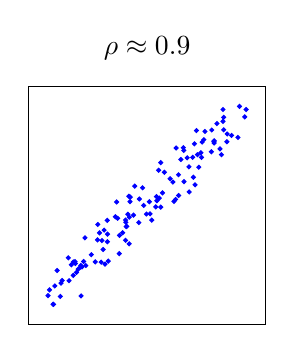
\begin{tikzpicture}
\begin{axis}[width=4.6cm,height=4.6cm,title={$\rho\approx0.9$},xtick=\empty,ytick=\empty,only marks,mark size=0.7pt]
\addplot[blue,only marks,mark=*,mark size=0.7pt,samples=120,domain=-2:2] ({x+0.4*rand},{x+0.4*rand});
\end{axis}
\end{tikzpicture}
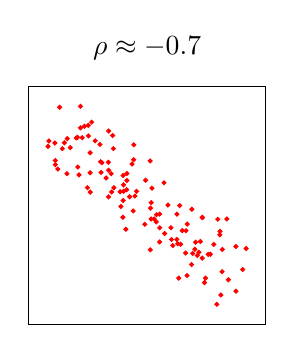
\begin{tikzpicture}
\begin{axis}[width=4.6cm,height=4.6cm,title={$\rho\approx-0.7$},xtick=\empty,ytick=\empty]
\addplot[red,only marks,mark=*,mark size=0.7pt,samples=120,domain=-2:2] ({x+0.6*rand},{-x+0.9*rand});
\end{axis}
\end{tikzpicture}
\begin{tikzpicture}
\begin{axis}[width=4.6cm,height=4.6cm,title={$\rho\approx0$ (مستقل)},xtick=\empty,ytick=\empty]
\addplot[gray,only marks,mark=*,mark size=0.7pt,samples=120,domain=-2:2] ({2*rand},{2*rand});
\end{axis}
\end{tikzpicture}
\begin{tikzpicture}
\begin{axis}[width=4.6cm,height=4.6cm,title={$\rho=0$ (وابسته!)},xtick=\empty,ytick=\empty]
\addplot[green!50!black,only marks,mark=*,mark size=0.7pt,samples=120,domain=-1:1] ({x},{x*x+0.05*rand});
\end{axis}
\end{tikzpicture}
\end{center}

\begin{note}
\notetitle تنها در حالت \textbf{مشترکاً گاوسی} است که ناهمبستگی و استقلال معادل‌اند (جلسه قبل، خاصیت ۲).
\end{note}

\section{تمرین‌های تکمیلی}

\begin{exercise}
در مثال جلسه سیزدهم با $f_{XY}=x+y$ روی مربع واحد، $\Cov(X,Y)$ و $\rho_{XY}$ را حساب کنید.
\end{exercise}
\begin{solution}
$\E X=\int_0^1x(x+\frac12)\dd x=\frac13+\frac14=\frac7{12}$ (و $\E Y$ نیز همین). $\E X^2=\int_0^1x^2(x+\frac12)\dd x=\frac14+\frac16=\frac5{12}$؛ پس $\sigma_X^2=\frac5{12}-\frac{49}{144}=\frac{11}{144}$.
$\E(XY)=\int_0^1\!\int_0^1xy(x+y)\dd x\dd y=\frac16+\frac16=\frac13$.
$\Cov=\frac13-\frac{49}{144}=-\frac1{144}$ و $\rho=\frac{-1/144}{11/144}=-\frac1{11}\approx-0.09$ ــ همبستگی منفی ضعیف.
\end{solution}

\begin{exercise}
$X,Y$ با $\Var X=4$، $\Var Y=9$ و $\rho_{XY}=0.5$ داده شده‌اند. $\Var(2X-Y)$ را بیابید.
\end{exercise}
\begin{solution}
$\Cov(X,Y)=0.5\cdot2\cdot3=3$. $\Var(2X-Y)=4\cdot4+9-2\cdot2\cdot3=16+9-12=13$.
\end{solution}

\begin{exercise}
یک تاس سالم دو بار پرتاب می‌شود. $S$ مجموع و $D$ تفاضل دو عدد است. نشان دهید $S$ و $D$ ناهمبسته‌اند. آیا مستقل‌اند؟
\end{exercise}
\begin{solution}
$\Cov(X_1+X_2,X_1-X_2)=\Var X_1-\Var X_2+\Cov(X_2,X_1)-\Cov(X_1,X_2)=0$. پس ناهمبسته‌اند. اما مستقل نیستند: اگر $S=2$ باشد حتماً $D=0$ است، در حالی که $\Prob(D=0)=\frac16$.
\end{solution}

\begin{exercise}
نشان دهید برای هر متغیرهای $X_1,\ldots,X_n$:
$\Var\big(\sum_iX_i\big)=\sum_i\Var X_i+2\sum_{i<j}\Cov(X_i,X_j)$.
\end{exercise}
\begin{solution}
$\Var(\sum X_i)=\Cov(\sum_iX_i,\sum_jX_j)=\sum_{i,j}\Cov(X_i,X_j)$ (دوخطی بودن). جملات $i=j$ واریانس‌ها هستند و هر جفت $i\ne j$ دو بار ظاهر می‌شود. برای متغیرهای دوبه‌دو ناهمبسته (نه لزوماً مستقل!) این رابطه به $\sum\Var X_i$ کاهش می‌یابد.
\end{solution}
